\chapter{Optimisation de l'algorithme et ajout de "l'houache" de la "voiture"}
\begin{figure}[!ht]
    \centering
    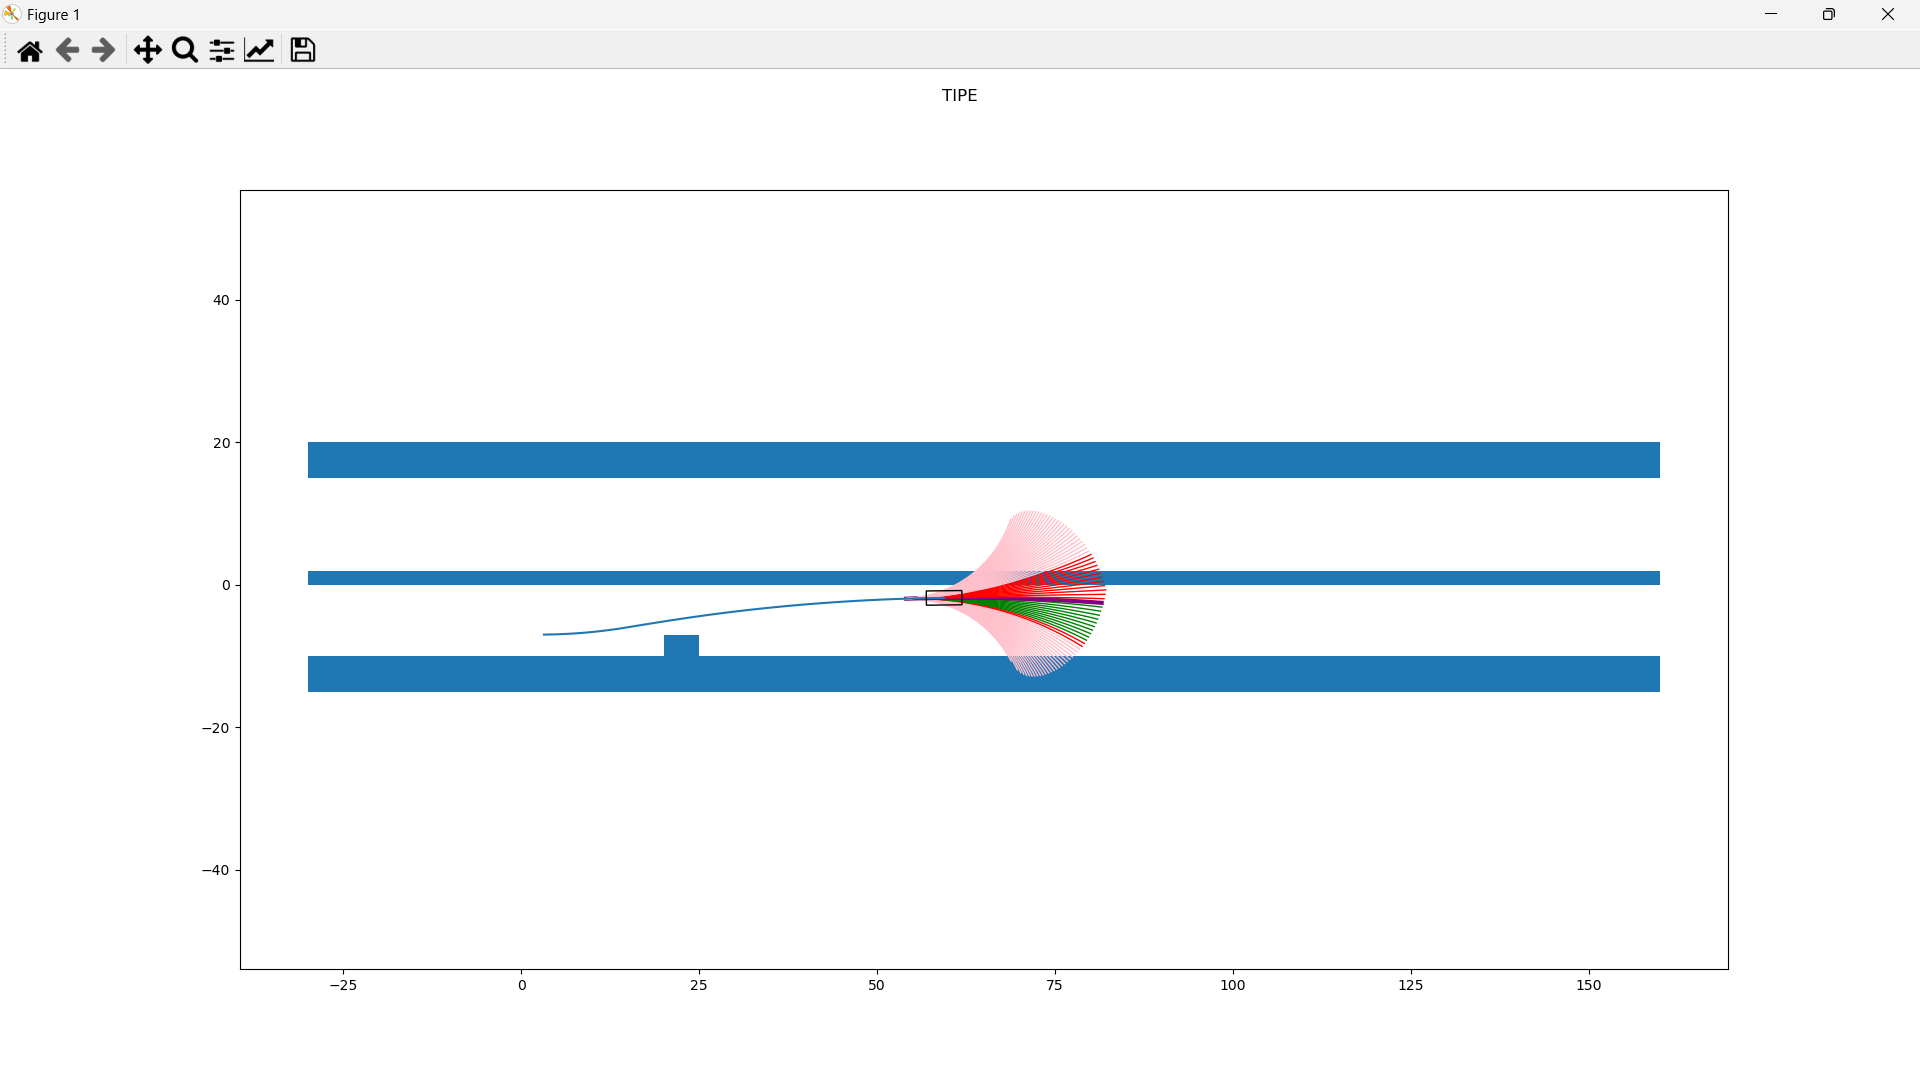
\includegraphics[scale=0.3]{evitement fin.png}
\end{figure}
\vspace{100pt}

\begin{mintedbox}{python}
"""
Déplacement de la voiture sur un parcours, en n'évaluant pas toutes les tentacules (gain de temps) et en affichant la trace de la voiture.
"""


class Voiture:
    """
    Objet voiture, défini par sa forme. D'autres paramètres fixes sont définis après, on pourra les mettre en paramètre plus tard si plusieurs voitures il y a.
    """
    def deplace(self):
        """
        S'il existe un chemin (suite de points), déplace la voiture suivant ce chemin.

        Raises
        ------
        erreur
            Le chemin à suivre n'est pas défini.

        Returns
        -------
        None.

        """
        try:
            new_x = self.chemin[1][0]
            new_y = self.chemin[1][1]
            vx = new_x - self.chemin[0][0]
            vy = new_y - self.chemin[0][1]
            new_angle = np.degrees(np.arctan2(vy, vx))
            self.shape_voiture.set(x=new_x - self.largeur/2, y=new_y - self.longueur/2, angle=new_angle)
            self.x, self.y, self.angle = new_x, new_y, new_angle
            self.chemin = np.delete(self.chemin, 0, 0)
            if self.traceur is True:
                self.trace.set_data(np.append(self.trace.get_data()[0], new_x), np.append(self.trace.get_data()[1], new_y))
        except IndexError:
            print('TENTACULE ÉPUISÉE, ON NE SAIT PLUS QUEL CHEMIN SUIVRE')

class Simulation_Ref_Terre:
    """
    Classe qui gère tout l'aspect simulation : animation + gestion des objets.

    Parameters
    ----------
    voitures: list
        Liste des voitures présentes
    obstaces: list  # TODO
        liste des obstacles FIXES. Ils ne seront pas animés
    obstacles_mvt: list  # TODO
        liste des obstacles à déplacer. Fonction dévelopée plus tard
    """
    def animer(self, i):
        """
        Anime la figure. S'occupe de déplacer les voitures et les obstacles.
        Note : fait appel au "task-manager des tentacules" pour savoir quoi actualiser dans la figure (blit)

        Parameters
        ----------
        i : int
            Numéro d'appel de la fonction (elle est censée être appelée itérativement par une matplotlib.animation.

        Returns
        -------
        list of artists
            Liste des dessins à actualiser (blit).

        """
        traces = []
        # Déplace les voitures
        for voiture in self.voitures:
            voiture.deplace()
        # Déplace les obstacles
        for obstacle in self.obstacles_mvt:
            obstacle.deplace()
        try:
            # Retourne la liste des dessins à actualiser dans la figure
            # TODO : ajouter les obstacles lors de l'import de la fonctionnalité
            return [voiture.shape_voiture for voiture in self.voitures] + [tentacule.patch for tentacule in self.new_tentacules] + [tentacule.patch for tentacule in self.old_tentacules] + [obstacle.patch for obstacle in self.obstacles_mvt] + [voiture.trace for voiture in self.voitures]
        finally:
            # Met juste après les valeurs adéquates à jour pour ne plus avoir à redessiner des dessins fixes (blit)
            self.old_tentacules = []  # Suppression des tentacules obsoletes, qu'on a bien effacé avec le return
            for tentac in self.old_tentacules:
                tentac.patch.remove()
            for tentac in self.new_tentacules:
                tentac.patch.set_animated(False)  # Dés-anime les nouvelles tentacules (affichées avec le return) : elles ne doivent plus bouger jusqu'à une redfinition de celles-ci. Sert ?

\end{mintedbox}
